\chapter{Class Diagrams and Interface Specifications}

\section{Class Diagram}
\begin{figure}[h]
\centering
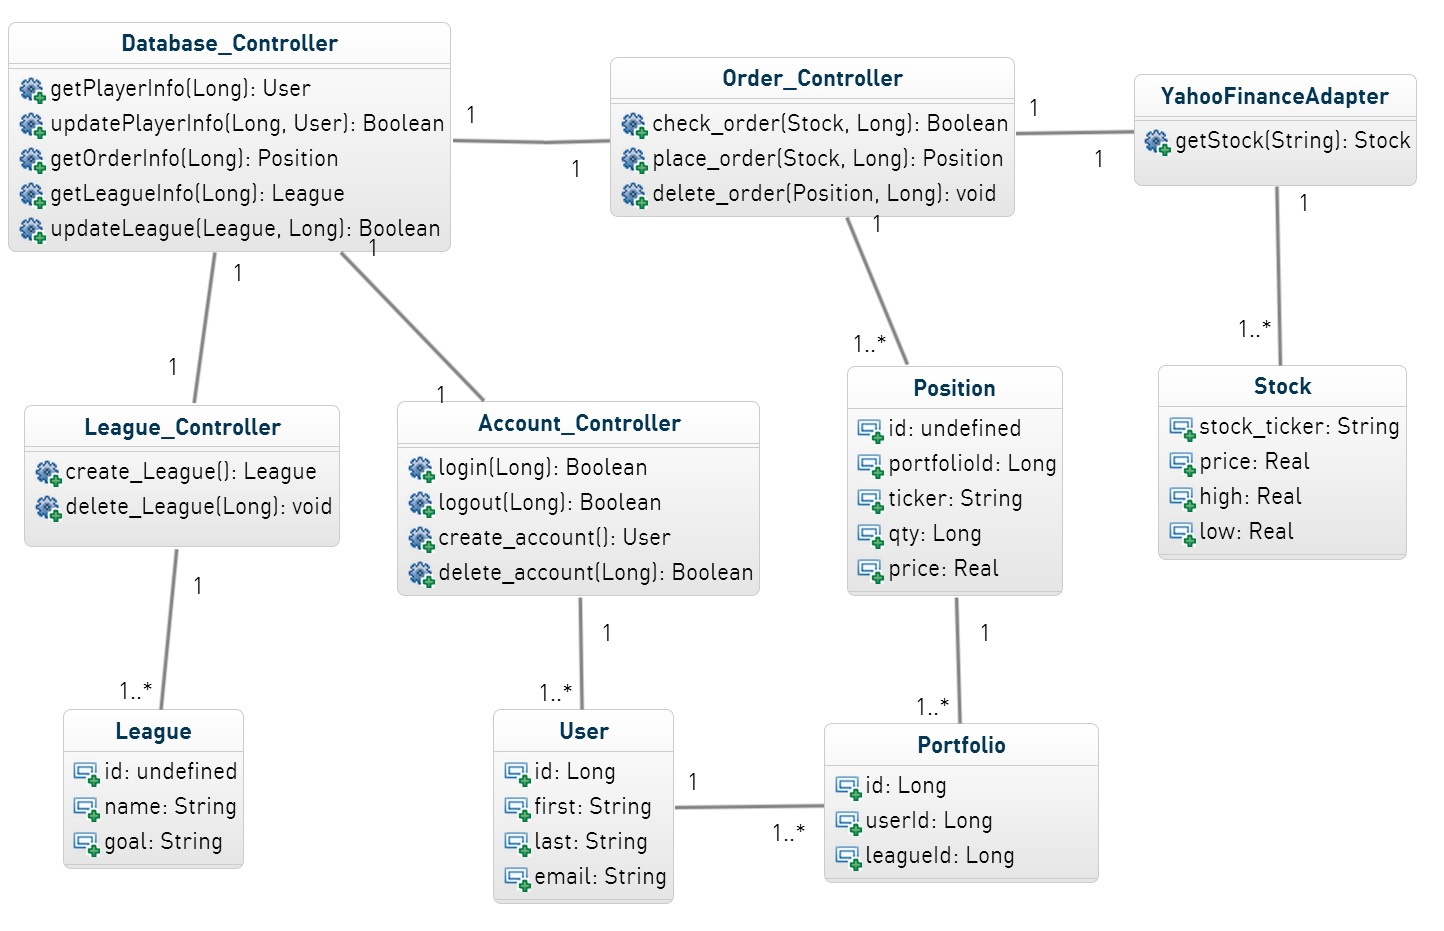
\includegraphics[width=5.5in]{./img/classDiagram.jpg}
\end{figure}


\clearpage

\section{Class Data Types and Operation Signatures}

\subsection{Database Manager}
Our database manager performs the function of managing the database. This can
mean anything from adding user information into the database, retrieving
information from the database and updating information in the database,
regardless of whether the information deals with users/accounts, leagues,
orders. \\*

{\bfseries Methods} \\*

{\bfseries + get_player_info(in user_id : long) : class User } \\*
	This method is used when information needs to be retrieved for a specifc
  player \\*

{\bfseries + update_player_info(in user_id : int, in upd: class user) : bool } \\*
    This method is used to update a user’s information, whether it be
    administrative or game related. \\*

{\bfseries + get_order_info(in transaction_id : int) : class transaction } \\*
	This method takes in a transaction id and returns the information associated
  with that specific transaction.\\*

{\bfseries + update_league(in league_id : int, in leagueInfo : class league) : bool } \\*
	This method returns the latest updates in the league \\*

{\bfseries + return_league_updates(in league_id : int) : class league  }\\*
This method is used when a league needs to be updated with the newest
information provided in the league in the input
	 \\*

\subsection{Order Manager}


Our order manager class is responsible for handling all the tasks related to
orders/transactions. It is responsible for placing the order in the system and
for moving old orders to the archive transactions table.
 \\* \\*

{\bfseries Methods} \\*

{\bfseries + Check_order(in symbols: class Order) : bool} \\*
This method is simple used to check and make sure that the input order can be
processed. It will check the users balance, etc.
     \\*

{\bfseries + place_order(in symbols: class Order) : bool } \\*
As the name suggests, this method is used to place an order in the system, with
the information given by the input Stock class.
	\\*

{\bfseries + delete_order(in symbols: transaction_id): bool } \\*
	As the name suggests, this method deletes an order from the system, assuming
  that it hasn’t already been processed. If it has then this function will
  return a false value.\\*

{\bfseries + Execute_order(in transaction_id : int) : bool } \\*
	This method is responsible for actually getting the stock
    information from Yahoo Finance API and then changing the
    account/portfolios to reflect it accordingly. \\*

\subsection{League Manager}

This class is responsible for managing all the leagues in the system. It has
the authority to create leagues, delete leagues, and modify leagues as it is
instruction to do so. \\* \\*

{\bfseries Methods} \\*

{\bfseries + Create_league () : Class league } \\*
	This function is used to create a league from scratch so that the user can
  create a league. \\*

{\bfseries + Delete_leagues(in league_id : int) : bool } \\*
	As the name suggests, this method will delete the league matching the input\\*

{\bfseries + change_league_name( in league_id : int) : bool } \\*
	This method is here solely for the purpose implied by its
    name.  It’s only function is to change the name of the
    league.  \\*

{\bfseries + Change_league_manager (in league_id : int, in usr : class User) : bool } \\*
	This function replaces the current league manager stored
    in the input league with the user specified in the input. \\*

{\bfseries + add_rules(in league_id : int) : bool } \\*
	This function is here for the reason its name suggests.
    It is here just to add rules to a given league.  \\*

{\bfseries + Delete_rules(in league_id : int) : bool } \\*
	This method exists just to delete the rules in a league.  \\*


\subsection{Account_Controller}
This class exists to take care of any function that relates to accounts. This
can mean creating an account, modifying an account, or even deleting
 \\* \\*

{\bfseries Methods} \\* \\*

{\bfseries + Login(in user_id : int) : bool} \\*
	This function is used by the user to log into the system

{\bfseries + logout(in user_id : int) : bool } \\*
	This function is the opposite to the one above it, it is
    used by the User to log out of the system. \\*

{\bfseries + Verify_User(in User_id : int) : bool} \\*
	Method to make sure that the person logging in or that
    the person who is logged in is not an imposter/fake. \\*

{\bfseries + Create_account() : class User } \\*
	Creates an account with the current user  \\*

{\bfseries + delete_account(in suser_id : int) : bool } \\*
	Used to delete an account from the database system.   \\*

\subsection{Yahoo Finanace Adapter}
This class is responsible for obtaining market data from Yahoo Finance
API.  It consists of 3 functions to get quotes, get company information,
and to get sector information.

{\bfseries Methods} \\* \\*

{\bfseries + Get_quote(in stock_ticker_id : string) : class quote } \\*
	As the name suggests, this method is responsible for obtaining
    quote information about a given stock_ticker \\*

{\bfseries + get_company_info(in stock_ticker_id : string) : class Company } \\*
	This method is responsible for getting market information about a
    specified company.  \\*

\subsection{Stock}
This class is responsible for representing a Stock. It has the authority to hold
a ticker symbol, price, daily high price, and daily low price. \\* \\*

{\bfseries Attributes} \\*

{\bfseries + String:stock_ticker} \\*
This attribute holds the ticker symbol as a character array.\\*
{\bfseries + double:price} \\*
This attribute holds the current value of stock corresponding to the ticker
symbol.\\*
{\bfseries + double:high} \\*
This attribute holds the current High price of the stock on the market.\\*
{\bfseries + double:low} \\*
This attribute holds the current Low price of the stock on the market.\\*

\subsection{User}
This class is responsible for representing a User. It has the authority to hold
first name, last name, email address, and userId.\\* \\*

{\bfseries Attributes} \\*

{\bfseries + long:id} \\*
A unique id to distinguish different users from one another. \\*
{\bfseries + String:first} \\*
This attribute holds the first name of the user. \\*
{\bfseries + String:last} \\*
This attribute holds the last name of the user. \\*
{\bfseries + double:low} \\*
This attribute holds the email address of the user. \\*


\subsection{Position}
This class is responsible for representing a Position, which is a stock that a
user owns. It has the authority to hold the user Id, portfolio Id, ticker
symbol, quantity and price.\\* \\*

{\bfseries Attributes} \\*

{\bfseries + long:id} \\*
A unique id to distinguish different users from one another. \\*
{\bfseries + long:portfolioId} \\*
A unique id to distinguish different users from one another. \\*
{\bfseries + String:ticker} \\*
This attribute holds the first name of the user. \\*
{\bfseries + long:qty} \\*
This attribute holds the quantity of the certain position.\\*
{\bfseries + double:price} \\*
This attribute holds the price that the position was purchased at.\\*

\subsection{Portfolio}
This class is responsible for representing a Portfolio, which is the set of
stocks that a user owns. It has the authority to hold the user Id, portfolio
Id, ticker symbol, quantity and price. \\* \\*

{\bfseries Attributes} \\*

{\bfseries + long:id} \\*
A unique ID to distinguish different portfolios from one another.\\*
{\bfseries + long:userId} \\*
A unique ID to distinguish who owns the portfolio. \\*
{\bfseries + String:leagueId} \\*
A unique ID to distinguish what league this portfolio is a part of. \\*

\subsection{League}
This class is responsible for representing a League, which is a group that
users can belong to, to compete with each other.\\* \\*

{\bfseries Attributes} \\*

{\bfseries + long:id} \\*
A unique ID to distinguish different portfolios from one another.\\*
{\bfseries + String:name} \\*
This attribute holds the name of the league.\\*
{\bfseries + String:goal} \\*
This attribute holds the necessary requirement for a person to be declared the
winner of a league. \\*

\section{Traceability Matrix}


\begin{figure}[H]
\centering
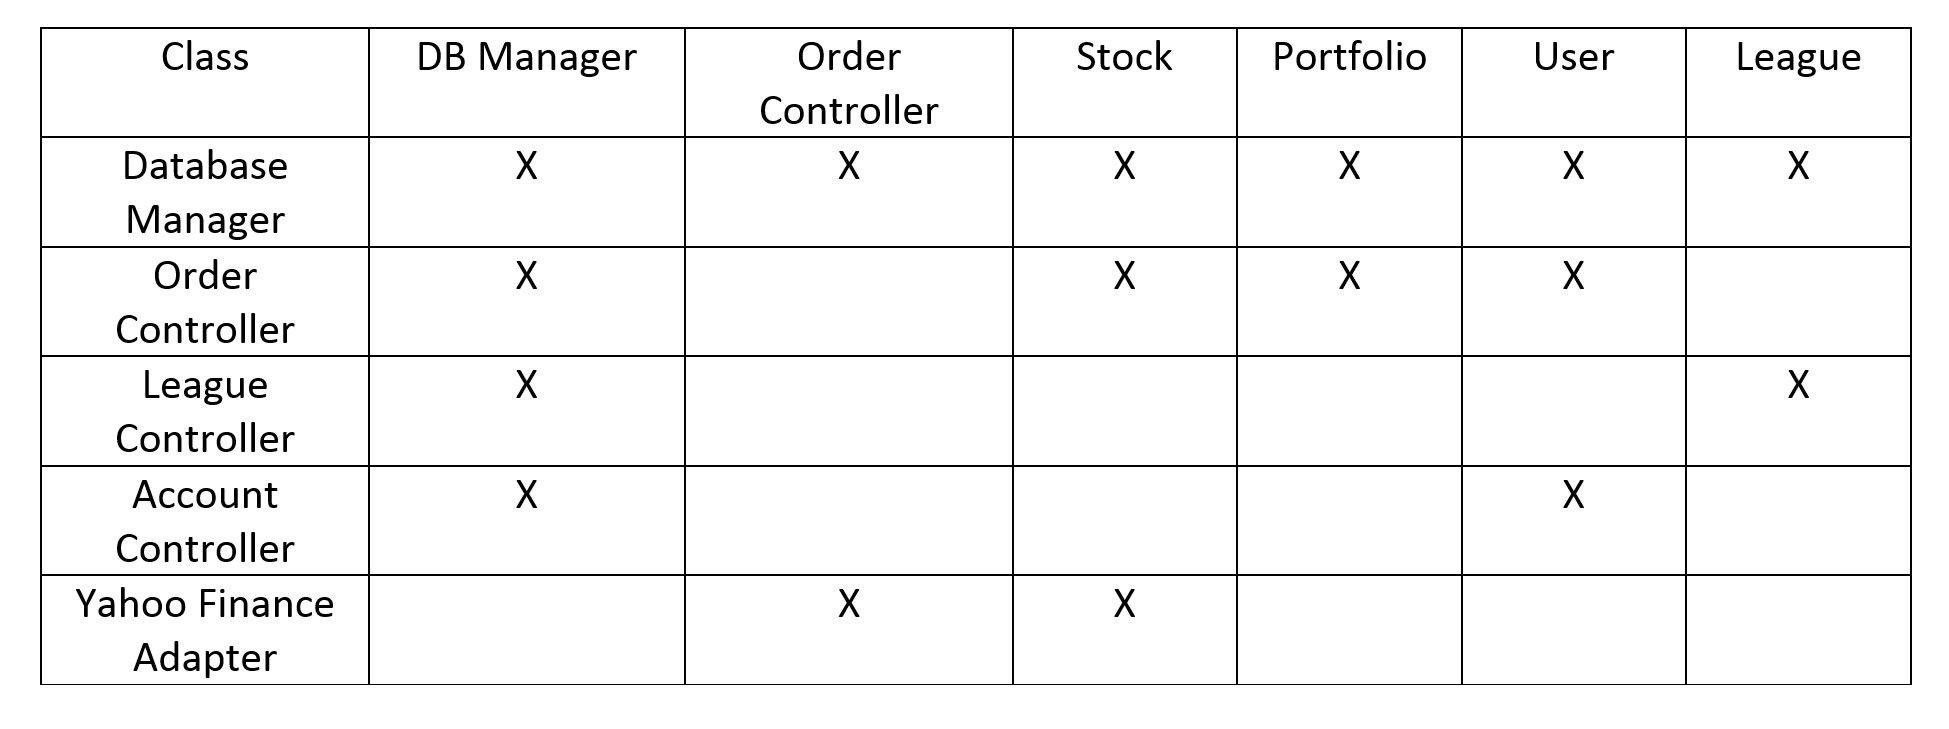
\includegraphics[width=5.5in]{./img/trace.jpg}
\caption{The database manager is in connection with all other controllers. This
is because all data is maintained in the database. The database also deals with
object classes such as Stock, Portfolio, User, and League. The order controller
only deals with Stocks and which portfolios to place them. The League Controller
only deals with leagues. The Account Controller deals with user objects. The
Yahoo Finance Adaptor returns Stock objects to the Order Controller when
requested.}
\end{figure}

\section{Object Constraint Language}

In order to separate ideas in OCL, we will split it up descriptions by each
class in the class diagram.

\subsection{Database Manager}
The data base manager is the central point where all data is recorded and
accessed. The existing constraints are as follows. When using a get[x]info()
function, the associated long id value must be available to be provided.
This allows access into the database tables to be able to return information
about a class. When using an update[x]() function, the associated long id must
be included, and also an object containing the information that you want to
update.

\subsection{Order Controller}
The order controller handles placing orders. The current constraint involved
with its functions require a portfolio id and Stock object.

\subsection{Yahoo! Finanace Class}

The Yahoo Finance Adapter is responsible for creating and returning a Stock
object based on the input data. The Yahoo Finance Server is contacted to
retrieve data. The constraint of this class is that proper Ticker symbols must
be input.

\subsection{Account Controller}
The account controller is able to create and delete accounts. The only
constraint to the account controller is that to delete an account the user id
must be available.

\subsection{League Controller}
The league controller is capable of creating and deleting leagues. There are no
constraints to creating a league. The only constraint to deleting a league is
that the league id must be available in the database, or in other words, the
league must exist.


